% !TeX spellcheck = fr_FR
\documentclass[12pt,a4paper]{report}
\usepackage{style/preambule_college}
\usepackage{style/preambule_personnalisation}
\usepackage{geometry}
\usepackage{amsmath}
\usepackage{tikz}
\usepackage{xcolor}
\usepackage{pgfplots}
\chapterFormat

\begin{document}
	
	\chapter[Analyse]{Les fonctions trigonométriques et leur réciproques}
	\section*{Fonctions trigonométriques}
	\subsection*{Sinus et cosinus}
	\subsubsection*{Définition et graphe}
	Il existe 2 fonctions trigonométrique principales: la fonction $\color{red}\cos(x)$ et $\color{blue}\sin(x)$.
	
	\begin{tikzpicture}
	\begin{axis}[
	domain=-10:10,
	xscale=2,yscale=1,
	xmin=-5, xmax=5,
	ymin=-1, ymax=1,
	samples=1000,
	axis lines=center,
	]
	\addplot+[mark=none,color=blue] {sin(deg(x))};
	\addplot+[mark=none,color=red] {cos(deg(x))};
	\end{axis}
	\end{tikzpicture}
	
	
	\subsubsection*{Propriétés}	
	\begin{enumerate}
	\item Ces 2 fonctions sont défini de $\mathbb{R}$ dans $[-1;1]$.
	\item Ce sont ces fonctions qui amènent la notion de période, en effet la fonction cosinus et sinus sont dites périodique car un morceau quelconque de la fonction se retrouve à l'identique dans tout le graphe. Ainsi on peut voir l'égalité $\cos(x+2\pi)=\cos(x)$ et $\sin(x+2\pi)=\sin(x)$. Ce qui veut dire que la fonction est de période $2\pi$.
	\item Ces fonctions ont également une parité qui, cette fois, est propre à chacun: le sinus est dit impair ($\sin(-x)=-\sin(x)$) et le cosinus est pair ($\cos(x)=\cos(-x)$).
	\end{enumerate}
	Une propriété intéressante qui fait un lien entre ces 2 fonctions sinus et cosinus: \[\sin(x)^2+\cos(x)^2=1\]
	
	\pagebreak
	\subsection*{Tangente}
	\subsubsection*{Définition et graphe}
	Une 3ème fonction trigonométrique appelée tangente et raccourcie en $\color{green}\tan$ est liée au cosinus et au sinus: \[\color{green}\tan(x) \color{black}=\dfrac{\color{blue}\sin(x)}{\color{red}\cos(x)}\]
	
	\begin{tikzpicture}
	\begin{axis}[
	domain=-1.5:1.5,
	xscale=0.5,yscale=1,
	xmin=-2.5, xmax=2.5,
	ymin=-5, ymax=5,
	samples=1000,
	axis lines=center,
	]
	\addplot+[mark=none,color=green] {tan(deg(x))};
	\end{axis}
	\end{tikzpicture}
	
	Cette fonction tire ses propriétés de l'égalité ci dessus.
	\subsubsection*{Propriétés}
	\begin{enumerate}
		\item Elle définie de $\mathbb{R} \backslash \{\frac{\pi}{2}+k\pi (k \in \mathbb{Z})\} $ dans $\mathbb{R}$.
		\item Elle a la même parité que la fonction sinus donc impaire: $\tan(-x)=-\tan(x)$.
		\item Elle a une période non pas de $2\pi$ mais de $\pi$. $\tan(x+\pi)=\tan(x)$.
	\end{enumerate}

	\pagebreak
	\section*{Fonction trigonométrique réciproque}
	\subsection*{Arcsin}
	\subsubsection*{Définition et graphe}
	La fonction $\sin(x)$ est définie pour tout réel $x$ mais ses images sont comprises dans l'intervalle $[-1;1]$ cette fonction est donc surjective. Pour définir sa fonction réciproque il faut rendre la fonction sinus bijective et donc restreinte l'ensemble de départ. On peut, par exemple, définir la fonction sinus de $[-\frac{\pi}{2};\frac{\pi}{2}]$ dans $[-1;1]$ et ainsi on cette fonction admet une réciproque appelée $\color{blue}\arcsin$ définie de $[-1;1]$ dans $[-\frac{\pi}{2};\frac{\pi}{2}]$.
	
	\begin{tikzpicture}
	\begin{axis}[
	domain=-1:1,
	xscale=1,yscale=1,
	xmin=-2, xmax=2,
	ymin=-2, ymax=2,
	samples=1000,
	axis lines=center,
	]
	\addplot[color=blue] {rad(asin(x))};
	\end{axis}
	\end{tikzpicture}
	\subsubsection*{Propriété}
	\begin{enumerate}
		\item La fonction $\arcsin$ est impaire.
		\item Une autre écriture utilisé est $\sin^{-1}(x)$.
	\end{enumerate}
	\subsection*{Arccos}
	\subsubsection*{Définition et graphe}
	La démarche effectuée pour la fonction $\sin$ sera la même que pour la fonction $\cos$. On redéfinit la fonction cosinus de $[0,\pi]$ dans $[-1;1]$, elle admet donc une réciproque arccos définie de $[-1;1]$ dans $[0,\pi]$.
	
	\begin{tikzpicture}
	\begin{axis}[
	domain=-1:1,
	xscale=0.7,yscale=0.7,
	xmin=-2, xmax=2,
	ymin=-0, ymax=3.5,
	samples=1000,
	axis lines=middle,
	]
	\addplot[color=red] {rad(acos(x))};
	\end{axis}
	\end{tikzpicture}
	
	\subsubsection*{Propriété}
	\begin{enumerate}
		\item La fonction arccos n'a pas de parité.
		\item Une autre écriture existe: $\cos^{-1}(x)$.
	\end{enumerate}
	\subsection*{Arctan}
	\subsubsection*{Définition et graphe}
	De nouveau la même démarche. La fonction $\tan(x)$ est périodique, on restreint le domaine à une période, donc la fonction est définie de $]-\frac{\pi}{2};\frac{\pi}{2}[$ dans $\mathbb{R}$. Elle devient bijective et admet donc une réciproque: $\arctan(x)$ définie de $\mathbb{R}$ dans $]-\frac{\pi}{2};\frac{\pi}{2}[$.
	
	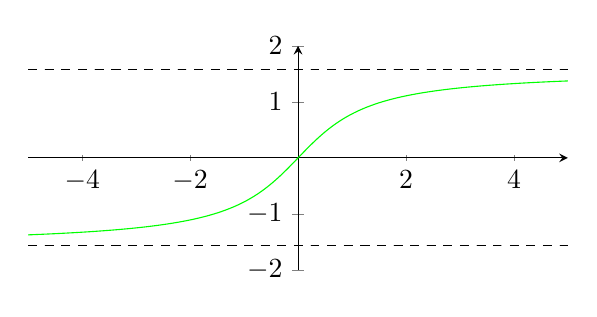
\begin{tikzpicture}
	\begin{axis}[
	domain=-5:5,
	xscale=1,yscale=0.5,
	xmin=-5, xmax=5,
	ymin=-2, ymax=2,
	samples=1000,
	axis lines=middle,
	]
	\addplot[color=green] {rad(atan(x))};
	\addplot[color=black,dashed] {pi/2};
	\addplot[color=black,dashed] {-pi/2};
	\end{axis}
	\end{tikzpicture}
	\subsubsection*{Propriété}
	\begin{enumerate}
		\item La fonction est impaire.
		\item Elle admet 2 limites: $\lim\limits_{x \rightarrow -\infty} \arctan(x)=-\dfrac{\pi}{2}$ et $\lim\limits_{x \rightarrow \infty} \arctan(x)=\dfrac{\pi}{2}$
	\end{enumerate}
	\section*{Dérivée}
	\subsection*{Cos-sin-tan}
	\[ (\cos(x))^{'}=-\sin(x)\] \[(\sin(x))^{'}=\cos(x)\] \[(\tan(x))^{'}=1+\tan(x)^2=\dfrac{1}{\cos(x)^2}  \]
	\subsection*{Fonction réciproque}
	$ (\arcsin(x))^{'}=\dfrac{1}{\sqrt{1-x^2}}$ (1) \hspace*{0.2cm} $(\arccos(x))^{'}=-\dfrac{1}{\sqrt{1-x^2}}$ (2) \hspace*{0.2cm} $(\arctan(x))^{'}=\dfrac{1}{1+x^2}$ (3)
	\subsubsection*{Démonstration}
	(1) $f(x)=y=\arcsin(x)$
	
	Par définition, on a: $\sin(y)=x$ \hspace{1cm} $ \forall x \in [-1;1]$
	
	En dérivant: $(\sin(y))'=(x)' \Leftrightarrow \cos(y)\cdot y'=1 \Rightarrow y'=\dfrac{1}{\cos(y)}$
	
	Comme $y=\arcsin(x) \in [-\dfrac{\pi}{2};\dfrac{\pi}{2}]$, on a $\cos(y) \geq 0 \Rightarrow \cos(y)=+\sqrt{1-(\sin(y))^2}$ c'est-à-dire $\cos(y)=\sqrt{1-x^2}$. On a donc:$y'=(\arcsin(x))'=\dfrac{1}{\displaystyle \sqrt{1-x^2}}$
	
	\vspace*{2cm}
	
	(2) la démarche est équivalente à la différence qu'un $-$ apparait. 
	
	$y'=(\arcsin(x))'=-\dfrac{1}{\sqrt{1-x^2}}$
	
	\vspace*{2cm}
	(3) $\tan(y)=x \forall x \in \mathbb{R}$ donc $(\tan(y))'=(x)'$
	
	$ \Rightarrow (1+\tan^{2}(y))\cdot y'=1 \Rightarrow y'=\dfrac{1}{1+\tan^{2}(y)} \Rightarrow y'=(\arctan(x))'=\dfrac{1}{1+x^2}$
	
\end{document}